\documentclass[11pt, oneside]{article}   	% use "amsart" instead of "article" for AMSLaTeX format
\usepackage{geometry}                		% See geometry.pdf to learn the layout options. There are lots.
\geometry{letterpaper}                   		% ... or a4paper or a5paper or ... 
%\geometry{landscape}                		% Activate for for rotated page geometry
%\usepackage[parfill]{parskip}    		% Activate to begin paragraphs with an empty line rather than an indent
\usepackage{graphicx}				% Use pdf, png, jpg, or eps� with pdflatex; use eps in DVI mode
								% TeX will automatically convert eps --> pdf in pdflatex		
\usepackage{amssymb}
\usepackage{amsmath}
\usepackage{parskip}
\usepackage{color}

\title{Escape and Orbital Velocity}
%\author{The Author}
%\section{}
% \subsection*{R code}
\date{}							% Activate to display a given date or no date

\graphicspath{{/Users/telliott_admin/Dropbox/Tex/png/}}

% \begin{center} 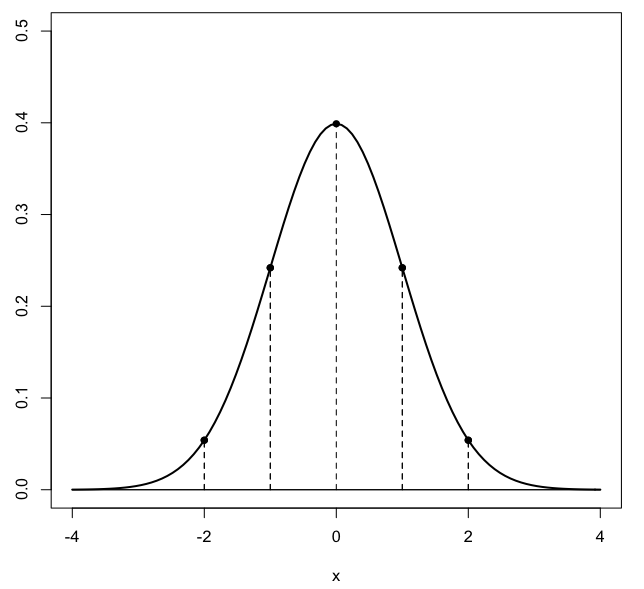
\includegraphics [scale=0.4] {gauss3.png} \end{center}

\begin{document}
\maketitle
\Large
\noindent

Here we want to think about problems related to the orbits of planets.  But let's start with a few simpler issues, the first of which is escape velocity.  We imagine an object starting from rest on the surface of the earth and then giving it enough velocity in the vertical direction so that it can move far enough that it is free from gravity altogether.  This last point is an approximation, but that's OK.

A simple approach is to use the principle of conservation of energy:  we will impart enough kinetic energy ($KE = (1/2) mv^2$) so that the increase in potential energy after the motion is just balanced.  The question is how to compute the potential energy.

In vector calculus we used this expression for work

\[ W = \int_C \mathbf{F} \cdot d \mathbf{r} \]

The work done over the course of the motion is equal to the energy obtained.  We can compute the work using the formula above, but we also recall that if the field $\mathbf{F}$ is the gradient of a scalar function (called the potential)

\[ \mathbf{F} = \nabla f \]

then a simpler method is to just evaluate $f$ at the start and end point and compute the difference.

\[ W = f(P_1) - f(P_0) \]

Here, $\mathbf{F}$ is the force of gravity

\[ \mathbf{F} = \frac{GM}{r^2} m \]

so our first task is to guess the form of the potential function.

\[ \nabla f = \frac{GM}{r^2} m \]

In Cartesian coordinates the gradient of $f$ is just 

\[ \nabla  = \frac{\partial f}{\partial x} \hat{\mathbf{i}} + \frac{\partial f}{\partial y} \hat{\mathbf{j}} + \frac{\partial f}{\partial z} \hat{\mathbf{k}}   = \ <f_x,f_y,f_z> \]

In radial coordinates it is a little trickier.  Let's sidestep that issue by just remembering that we are moving in only one direction, straight up, so we can use the Cartesian version.  We look for a function whose derivative is the force

\[  \frac{\partial f}{\partial r} = \frac{GM}{r^2} m \]
\[ f = -\frac{GM}{r} m \]

an elementary result from differential calculus.  So the potential difference between $r = R \rightarrow \infty$ (where $R$ is the radius of the earth), is

\[ W = f(P_{\infty}) - f(P_E) \]
\[ = -\frac{GM}{R} m  \bigg |_R^{\infty} \]
\[ = 0 + \frac{GM}{R} m \]
\[ = \frac{GM}{R} m \]

I may have a sign error here.  The physicists define things backwards compared to the mathematicians.  If in doubt, take the absolute value of the energy.  :)

So that is how much kinetic energy we need to impart.  Using the standard form for KE, this leads to 

\[ \frac{1}{2}mv^2 = \frac{GM}{R} m \]
\[ \frac{1}{2}v^2 = \frac{GM}{R} \]
\[ v = \sqrt{ \frac{2GM}{R}} \]

The velocity needed is independent of the object's mass (though of course it will take more energy to get a bigger object from zero up to a certain velocity).  The velocity needed is called the escape velocity.

\subsection*{Kline}

Morris Kline uses a different approach.  We start with the acceleration due to gravity

\[ a = -\frac{GM}{r^2} \]

The minus sign is  because $a$ points down, but $r$ increases going up.  Write this explicitly as the derivative of position with respect to time

\[ \frac{d^2 r}{dt^2} = -\frac{GM}{r^2} \]

Now, he says, we'd like to integrate both sides (with respect to $t$, naturally).  That would give us $v(t)$ on the left.  But what is written on the right is not explicitly a function of time.  What to do?  

Use the chain rule!  Manipulating the left-hand side:

\[ \frac{d^2 r}{dt^2} = \frac{dv}{dt} = \frac{dv}{dr} \frac{dr}{dt} = v \frac{dv}{dr} \]

Clever, eh?  Hence

\[ v \frac{dv}{dr} = -\frac{GM}{r^2} \]

Moving $dr$ to the right-hand side and integrating, we obtain

\[ \frac{v^2}{2} = \frac{GM}{r} + C \]

You may recognize a connection between kinetic and potential energy here, we are just missing the mass $m$.

We can evaluate the constant $C$ by recognizing that we want $v=0$ for some particular $r$ that we're going to choose.  It may be $r \rightarrow \infty$ as we had above, or it might be some other $r$.  

What we could do is just to deal with the velocity and the radius at the two points, subtract, and then the constant goes away.

\[ \frac{v_2^2}{2} -  \frac{v_1^2}{2} = \frac{GM}{r_2} - \frac{GM}{r_1}  \]

Then if $v_2 = 0$ and $r_2 = R$,  and $r_1 = \infty$

\[ -  \frac{v_1^2}{2} = \frac{GM}{R}   \]

I definitely have a sign error here.  But it is basically the same as what we had before.

OTOH, let's call the radius where $v=0$, $r_{1}$.  There

\[ 0 = \frac{GM}{r_{1}} + C \]
\[ C = -\frac{GM}{r_{1}}  \]
\[ \frac{v^2}{2} = \frac{GM}{r} -\frac{GM}{r_{1}} \]

Now ask what happens in the limit as $r_1 \rightarrow \infty$, and the $r$ of interest to us is the radius of the earth $R$

\[ \lim_{r_1 \rightarrow \infty}  \frac{GM}{r_1} = 0 \]
\[ \frac{v^2}{2} = \frac{GM}{R}  \]

and this is the same result as we had before.  Let's calculate $v$

\[ G = 6.67384 \times 10^{-11} \ \text{m}^3 \ \text{kg}^{-1} \ \text{s}^{-2} \]
\[ R = 6.371 \times 10^{6} \ \text{m} \]
\[ M = 5.97219 \times 10^24 \ \text{kg} \]
\[ v = 11185 \ \text{m} / \text{s} \]

Just a touch over $25,000$ miles per hour.

\subsection*{Kline II}

Kline also uses a different argument to achieve the same goal.

\[ \frac{d^2 r}{dt^2} = -\frac{GM}{r^2} \]

Multiply both sides by 

\[ \frac{dr}{dt} \cdot \frac{d^2 r}{dt^2} = -\frac{GM}{r^2} \cdot  \frac{dr}{dt} \]

Now, the derivative is just a function.  Pretend we don't know what it is, call it $u$, and substitute the left-hand side \emph{only}.

\[ u = \frac{dr}{dt} \]
\[ u \ \frac{du}{dt} = -\frac{GM}{r^2} \cdot  \frac{dr}{dt} \]

Now, multiply by $dt$ and integrate.  Or if you prefer, reverse the chain rule and integrate both sides with respect to $t$.

\[ \frac{1}{2} u^2 =  \frac{GM}{r} + C \]

Recall that $u$ is really just $v$

\[  v = \frac{dr}{dt} = u \]
\[ \frac{1}{2} v^2 =  \frac{GM}{r} + C \]

A bit of sleight of hand.

\end{document}  